\documentclass[preprint,superscriptaddress,amsmath,amssymb,aps,prl]{revtex4-1}

\usepackage{graphicx}
\usepackage{xcolor}

\newcommand{\add}[1]{\textcolor{blue}{#1}}
\newcommand{\remove}[1]{\textcolor{red}{(#1)}}

\begin{document}


\title{Phonon lasing from optical frequency comb illumination of trapped ions}

\author{Michael Ip}
\email{michaelip9228@physics.ucla.edu}
\affiliation{University of California Los Angeles}
\author{Anthony Ransford}
\affiliation{University of California Los Angeles}
\author{Andrew M. Jayich}
\affiliation{University of California Santa Barbara}
\author{Xueping Long}
\affiliation{University of California Los Angeles}
\author{Conrad Roman}
\affiliation{University of California Los Angeles}
\author{Wesley C. Campbell}
\affiliation{University of California Los Angeles}


\date{\today}

\begin{abstract}
We demonstrate the use of a resonant, frequency-doubled optical frequency comb as an alternative to ultraviolet (UV) or even deep UV continuous-wave lasers to load, cool, and crystallize trapped atomic ions.  Since the frequency comb has teeth on both sides of atomic resonance, this introduces the complication that amplification of the atom's motion can be driven as well as cooling.  However, we find that the Doppler shift from the atom's oscillation introduces additional cooling that balances the amplification and gives rise to steady-state lasing of the ion's harmonic motion in the trap.  The gain saturation of this phonon laser keeps the optical frequency comb from continually adding energy without bound, and this protection allows us to demonstrate loading and crystallization of hot ions directly with the comb, a technique that is extendable to the deep UV.
\end{abstract}

\maketitle

The outermost valence electrons in atomic ions are tightly bound to the electron-shielded nucleus ($q_\mathrm{eff} \gtrapprox +2e$), and therefore typically require laser light in the ultraviolet (UV) for Doppler cooling \cite{Wineland1975proposed,Hansch1975cooling,Neuhauser1978optical,Wineland1978radiation}.  This is particularly problematic for species requiring light at wavelengths shorter than $\lambda \approx 204 \mbox{ nm}$ \cite{Kato1986second}, which includes $\mathrm{Hg}^+$ \cite{Oskay2006singleatom,Rosenband2008frequency}, $\mathrm{Al}^+$ \cite{Schmidt2005spectroscopy,Dai2015vacuum}, $\mathrm{He}^+$ \cite{Herrmann2009feasibility,Cingoz2012direct}, and highly-charged ions \cite{Nauta2017towards}.  While continuous-wave (cw) laser light is challenging to produce in the UV and deep UV (DUV), mode-locked (ML) lasers can be easily converted to short wavelengths due to their high instantaneous intensity \cite{McPherson1987studies,Porat2017phase}. This makes ML lasers attractive alternatives for working with ions, but their inherently complicated spectra (optical frequency combs) can lead to deleterious effects such as motional amplification instead of damping.

Despite this, the promise of having appreciable coherent optical power at challenging wavelengths has driven research in optical frequency comb laser cooling \cite{Blinov2006broadband,Kielpinski2006laser,DavilaRodriguez2016doppler,Jayich2016direct}. %, particularly in the resolved comb tooth regime where a single tooth can Doppler cool atoms much like a single cw laser. However, to maximize the scattering force, the excited state lifetime of the cycling transition ($\tau$) should be comparable to the repetition period of the laser ($T_\mathrm{r}$) \cite{Blinov2006broadband}, which violates the condition necessary for being in the fully-resolved tooth limit ($\tau \gg T_\mathrm{r}$) and raises the possibility that amplification of motion by blue-detuned light will make cooling  (and, in particular, loading and crystallization \cite{DavilaRodriguez2016doppler}) impractical.
 The two approaches that have been demonstrated for ions relied on ultraviolet cw lasers to pre-cool and pre-trap the ions before introducing the comb, thereby limiting the bandwidth that could be Doppler shifted into resonance. In the ``broadband laser'' regime \cite{Blinov2006broadband} (where the excited state lifetime of the atomic cycling transition is shorter than the laser repetition period, $\tau < T_\mathrm{r}$), Doppler cooling was performed by positioning the laser's center frequency to the red side of resonance.  Cooling was observed and presented with a theoretical model based on the shape of the single-pulse spectrum (as opposed to a frequency comb) that predicted a minimum achievable temperature of $T_\mathrm{min}=3.4\mbox{ K}$.  However, the cooled radial mode of motion in that work reached $1\mbox{ K}$, and the axial mode reached a temperature more than an order of magnitude colder than the broadband theory. We show here that even in this regime ($\tau \approx \frac{1}{4}T_\mathrm{r}$), significant comb tooth effects persist that can explain these anomalously low temperatures.  In another approach  \cite{DavilaRodriguez2016doppler}, the motional amplification by blue-detuned teeth was avoided by moving them far away from resonance by using a high-repetition-rate ($1/T_\mathrm{r} = 373 \mbox{ MHz} $) laser.  The frequency comb in that work was unable to crystallize initially hot ions, and several improvements were suggested for achieving this goal, including further shortening the repetition period of the laser to move the neighboring teeth even further from resonance \cite{DavilaRodriguez2016doppler}. 

In this Letter, we show that multi-tooth effects protect the ion from unbounded motional amplification and permit practical loading, cooling, and crystalization of hot ions directly with frequency combs, eliminating the need for UV cw lasers. By making use of a frequency comb that is able to achieve intensities of order $I_\mathrm{sat}$ for each tooth, we are able to observe and manipulate the ion's behavior even when it is not cooled to crystallization.  We find that instead of heating the ion out of the trap, the interaction with multiple comb teeth gives rise to stable phonon lasing of the ion's motion \cite{Vahala2009a,Xie2013pulsed}, an interpretation that is confirmed by the observation of injection locking of the ion's amplified mechanical oscillation \cite{Knunz2010injection}. Irrespective of the sign of detuning for the comb tooth closest to resonance, saturable vibrational lasing leads to a comb of stable, fixed-point oscillation amplitudes maintained by cooperative effects between red- (cooling) and blue-detuned (amplifying) comb teeth.  We find that ions in high-amplitude fixed points can be probabilistically transferred to lower amplitude fixed points by scanning the detuning, thereby allowing them to be cooled into the lowest fixed point and crystallized.  We also present a theoretical model of this behavior that agrees with our observations, and provide an expression for the achievable Doppler limit for laser cooling with optical frequency combs.

Single ${}^{174}\mathrm{Yb}^+$ (or ${}^{171}\mathrm{Yb}^+$) ions for this work are confined in a radio-frequency (rf) Paul trap with oblate spheroidal symmetry \cite{Yoshimura2015creation}, driven by a sinusoidal voltage at $\Omega_\mathrm{rf} = 2 \pi \times 48.535\mbox{ MHz}$.  The secular frequencies of motion are typically $(\omega_x,\omega_y,\omega_z) \approx 2 \pi \times (550,500,920)\mbox{ kHz } (\pm 2 \pi \times 10 \mbox{ kHz})$. We illuminate the ions with laser beams that are confined to the $xy$-plane and $\omega_x$ is the frequency of the phonon mode that lases most frequently due to the fact that it is closest to parallel to the ML laser propagation direction ($\Delta \theta = 23^\circ \pm 2^\circ$, see Fig.~\ref{fig:WideCombScan}). Fluorescence emitted in the $-z$ direction is collected by an imaging system and recorded on a photon-counting photomultiplier tube (PMT) and intensified CCD camera through a $369 \mbox{ nm}$ bandpass filter.

The ML laser for this work is a commercial picosecond Ti:sapphire laser oscillator \footnote{SpectraPhysics Tsunami} with a repetition rate of $f_\mathrm{r} = 1/T_\mathrm{r} = 81.553\mbox{ MHz}$.  The center frequency of the laser is set near $405.645\mbox{ THz}$, and the output is frequency doubled via single-pass through  a $0.8\mbox{ cm}$ LBO crystal cut for Type I phase matching for SHG of 760\mbox{ nm} light, generating an average UV power of around $9\mbox{ mW}$ at $\lambda \approx 369.5\mbox{ nm}$.  The laser bandwidth ($> 10 \mbox{ GHz}$) far exceeds the natural linewidth ($\gamma \equiv 1/\tau = 2 \pi \times 19.7\mbox{ MHz}$) and Zeeman splitting ($< 5 \mbox{ MHz}$) of the ${}^2P_{1/2} \leftrightarrow {}^2S_{1/2}$ transition in $\mathrm{Yb}^+$.  The peak ion fluorescence observed indicates that the optical power per comb tooth at the ion is $\approx 1.4 \mbox{ }\mu\mbox{W}$.  For all of the experiments reported here, we simultaneously illuminate the trapped ion with the mode-locked laser at $369.5\mbox{ nm}$ and a cw repump laser at $935\mbox{ nm}$ that has no observable direct mechanical effect on the ion.

For these parameters, the probability that an excited ion decays between pulses is $P_\mathrm{decay}(\gamma, T_\mathrm{r}) \equiv (1 - \mathrm{e}^{-\gamma T_\mathrm{r}}) = 78$\%. Quantitatively, the quasi-steady-state scattering rate for an atom at rest illuminated by a resonant comb of uniformly intense teeth ($\tau_\mathrm{pulse} \ll T_\mathrm{r}$) is given by \cite{Felinto2003coherent,Ilinova2011doppler,Aumiler2012simultaneous}
\begin{equation}
\Gamma_\mathrm{comb}(\delta) = \frac{1}{T_\mathrm{r}}\frac{\sin^2\left( \frac{\theta}{2} \right) \sinh \left( \frac{\gamma T_\mathrm{r}}{2}\right)}{\cosh \left( \frac{\gamma T_\mathrm{r}}{2}\right)- \cos^2\left( \frac{\theta}{2} \right)\cos (\delta T_\mathrm{r})},\label{eqn:barecomb}
\end{equation}
where $\delta$ is the angular detuning of a reference tooth from resonance ($\delta \equiv \omega_\mathrm{tooth} - \omega_\mathrm{atom}$) and $\theta$ is the pulse area, defined as the integral of the instantaneous Rabi frequency for a single pulse, $\theta \equiv \int\mathrm{d}t \Omega(t)$.

We quantify the relative importance of considering a comb-like vs.\ broadband (single-pulse) spectrum by the tooth visibility $V \equiv (\Gamma_\mathrm{max} - \Gamma_\mathrm{min}) / (\Gamma_\mathrm{max} + \Gamma_\mathrm{min})$, where $\Gamma_\mathrm{min}\equiv\Gamma_\mathrm{comb}(\frac{\pi}{T_\mathrm{r}})$ and $\Gamma_\mathrm{max}\equiv\Gamma_\mathrm{comb}(0)$ are the minimum and maximum scattering rates in the steady-state spectrum.  From Eq.~\ref{eqn:barecomb}, we find
\begin{equation}
V = \cos^2\left( \frac{\theta}{2}\right) \mathrm{sech}\left( \frac{\gamma T_\mathrm{r}}{2}\right),\label{eqn:Visibility}
\end{equation}
which shows that phase-coherent, inter-pulse effects persist remarkably far into the $\tau < T_\mathrm{r}$ regime, tracking the decay of the off-diagonal elements of the density matrix (i.e.\ the coherences) more closely than the populations.  For instance, the lifetime-limited ($\theta \!\!\rightarrow \!\!0$) tooth visibility in this work is $V=0.77$ despite the fact that more than $3/4$ of the excited state population decays between pulses.

Figure \ref{fig:WideCombScan}(a) shows the $369.5\mbox{ nm}$ fluorescence collected from a trapped ion as the teeth of the optical frequency comb illuminating it are scanned. The dashed gray curve is given by Eq.~\ref{eqn:barecomb}, and has been adjusted for the overall vertical scale (with no offset) and is shown for $\theta = 0.38\, \pi$, yielding a measured tooth visibility of $V=0.53$. The data are taken for $100 \mbox{ ms}$ of illumination per point so that the ion's motional temperature reaches steady-state for each frequency shown, and background counts $(\approx 170 \mbox{ kcps})$ have been subtracted by taking the difference between the PMT signal with and without the $935 \mbox{ nm}$ repump laser.

\begin{figure}
\begin{center}
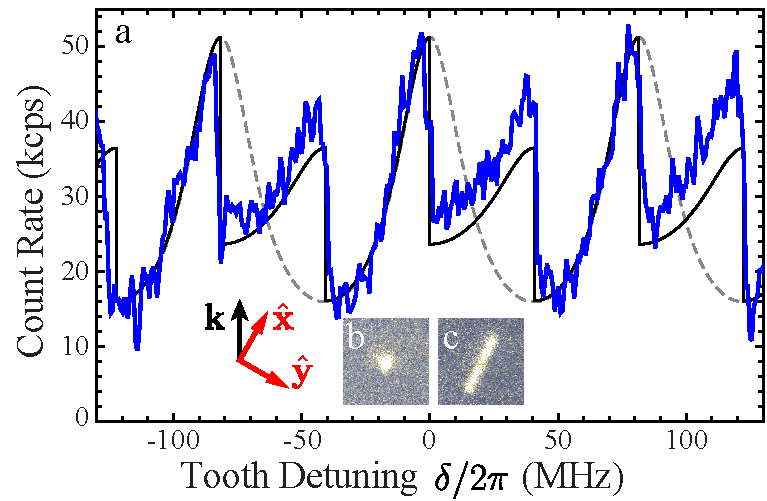
\includegraphics[width=1.0\columnwidth]{Fluorescence_Wide_Comb_Scan_07.pdf}
\end{center}
\caption{Fluorescence spectrum (in kilocounts per second) from a single trapped ion illuminated by an optical frequency comb.  When the near-resonant tooth is red detuned, the ion is localized via Doppler cooling (b) and the spectrum (a) follows the rest-frame lineshape from Eq.~\ref{eqn:barecomb} (dashed, gray).  When the near-resonant tooth is blue detuned, the ion oscillates with a fixed amplitude (c) and the fluorescence shows clear departure from the natural rest-frame resonance shape.  The solid black curve is $\Gamma(\delta,x_0)$ with oscillation amplitude $x_0=0$ or $x_0=4.9\mbox{ }\mu\mbox{m}$ when the near-resonant comb tooth is red or blue detuned, respectively.  The systematic increase in count rate from left to right is consistent with laser drifts during the measurement.}
\label{fig:WideCombScan}
\end{figure}

The fluorescence in Fig.~\ref{fig:WideCombScan}(a) tracks the ion's (power-broadened) rest-frame lineshape (Eq.~\ref{eqn:barecomb}) well when the near-resonant tooth is on the red side of atomic resonance ($\delta < 0$). As the near-resonant tooth crosses resonance and becomes blue-detuned ($\delta>0$), the fluorescence no longer follows the rest-frame prediction of Eq.~\ref{eqn:barecomb}, and an additional peak appears. As shown in Fig.~\ref{fig:WideCombScan}(c), the ion in this case oscillates with a large amplitude ($x_0=(4.9 \pm 0.5) \mbox{ }\mu\mbox{m}$).

To model the fluorescence spectrum of an ion oscillating slowly ($\omega_x \ll \gamma$) with fixed secular amplitude $x_0$, we calculate the average of the atomic scattering rate over a secular oscillation period in the trap ($T_\mathrm{sec} \equiv 2 \pi/\omega_x$): $\Gamma(\delta,x_0) \equiv \langle \Gamma_\mathrm{comb} \rangle_{T_\mathrm{sec}}$  \cite{SupplementalMaterials}.
%Since $\Omega_\mathrm{rf}\!>\!\!\,\gamma$, we include the effects of rf micromotion as an incoherent sum over the scattering rates from secular-phase-dependent micromotion sidebands \cite{Blumel1989chaos}, with each sideband yielding fluorescence with the functional form of Eq.~\ref{eqn:barecomb}.  Defining $\xi \equiv \omega_x t$, the secular-cycle-averaged scattering rate is given by
%\begin{equation}
%\Gamma(\delta, x_0) = \frac{1}{2 \pi} \int_0^{2 \pi} \mathrm{d}\xi \sum_n \mathrm{J}_n^2\!\left[ k x_0 \frac{q}{2} \cos(\xi)\right]\Gamma_\mathrm{comb} \left(\delta + n \Omega_\mathrm{rf} + k \omega_x x_0 \sin(\xi) \right)\label{eqn:Gamma}
%\end{equation}
%where $q\approx 2 \sqrt{2}\omega_x/\Omega_\mathrm{rf}$ is the Mathieu $q$-parameter for this normal mode, $k$ is the projection of the laser's k-vector on the oscillation axis, and $\mathrm{J}_n[\alpha]$ is the $n$th Bessel function of the first kind.
The black curve in Fig.~\ref{fig:WideCombScan} shows the scattering rate predicted by this model (scaled for the overall signal height) with a constant oscillation amplitude of $x_0=4.9 \mbox{ }\mu\mbox{m}$ when the nearest-resonant tooth is on the blue side of resonance and $x_0=0$ on the red side.  The asymmetric extra peak appearing blue of resonance is due to the shape of the cycle-averaged spectrum (which has a micromotion sideband at $+\Omega_\mathrm{rf}$, see Supplemental Materials \cite{SupplementalMaterials}) and the abrupt transition to a localized ion when the near-resonant tooth switches between blue and red detuning. 

The explanation for why the ion oscillates with large amplitude lies in a nonlinear, multi-tooth effect.  A trapped ion illuminated by two colors of cw laser light (one red- and the other blue-detuned) can be mapped onto a van der Pol oscillator \cite{Vahala2009a,Knunz2010injection,Lee2013quantum}, a prototypical, self-sustained oscillator model that can arise in the description of optical lasers \cite{Yariv1974frequency}.  The blue-detuned cw laser light can drive stimulated emission of phonons, and its experimental observation was reported as a phonon laser \cite{Vahala2009a}.

In the case studied here, the ML comb teeth all have nearly the same strength and there are hundreds, as opposed to two frequencies. To model this system, we work with secular-cycle-averaged expressions for the secular energy $E\equiv \frac{1}{2}m \omega_x^2 x_0^2$, amplitude damping coefficient $\beta(E)$, and stochastic heating rate $S(E)$ from spontaneous emission and the randomness in absorption.  The rate of energy transfer from the optical comb to the ion's motion is given by
\begin{equation}
\frac{\mathrm{d}E}{\mathrm{d}t} = -\beta(E) \frac{2E}{m} + S(E). \label{eqn:PowerBalance}
\end{equation}
The stochastic heating power can be calculated from the cycle-averaged scattering rate, $S(E) = (1 + \zeta)\frac{\hbar^2 |\mathbf{k}|^2}{2 m} \Gamma(\delta, x_0)$, where $\zeta = \frac{2}{5}$ is the geometric factor for dipole emission \cite{Leibfried2003quantum} and $x_0 = \sqrt{2E/m \omega_x^2}$.  The coherent (i.e.~non-stochastic) amplification power is given by $-\beta 2 E/m = \left\langle\mathbf{F}\cdot \mbox{\boldmath$v$}_\mathrm{sec}\right \rangle_{T_\mathrm{sec}}$, where $\mathbf{F} = \hbar \mathbf{k} \Gamma_\mathrm{comb}$ and $\mbox{\boldmath$v$}_\mathrm{sec}(t)$ is the instantaneous secular velocity \cite{SupplementalMaterials}.
%This yields an expression for the amplitude damping coefficient,
%\begin{equation}
%\beta(E) = \frac{\hbar k}{2 \pi \omega_x x_0} \int_0^{2 \pi} \mathrm{d}\xi \sin(\xi) \sum_n \mathrm{J}_n^2\!\left[ k x_0 \frac{q}{2} \cos(\xi)\right]\Gamma_\mathrm{comb} \left(\delta + n \Omega_\mathrm{rf} + k \omega_x x_0 \sin(\xi) \right).\label{eqn:Beta}
%\end{equation}

\begin{figure}
\begin{center}
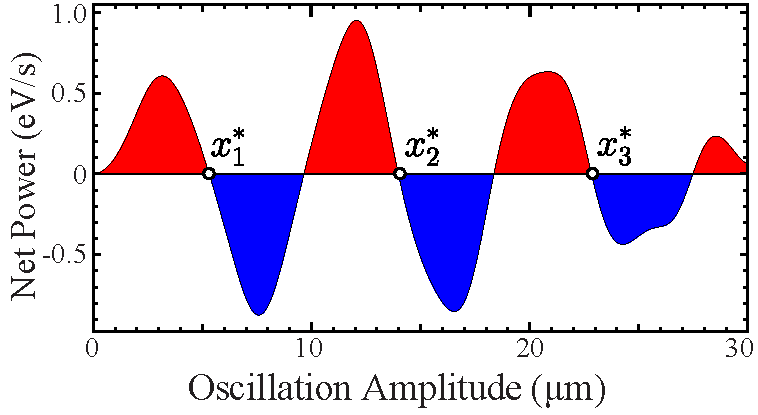
\includegraphics[width=1.0\columnwidth]{New_Theory_With_Everything_for_Paper_03.pdf}
\end{center}
\caption{Calculated net power delivered to the motion of a trapped $\mathrm{Yb}^+$ atom illuminated by an optical frequency comb as a function of the amplitude of the oscillations in the trap. The right side of Eq.~\ref{eqn:PowerBalance} is plotted for the case where the near-resonant tooth is blue-detuned with $\delta = \pi/2T_\mathrm{r}$.  Red (blue) shading indicates amplification (damping) of the ion's motion.  Stable fixed points are shown by circles. The red-detuned case ($\delta \! \rightarrow -\delta$) is similar but inverted with an additional fixed point near zero ($x_0^* = 90 \mbox{ }\mbox{nm}$).}
\label{fig:TheoryPowervsAmplitude}
\end{figure}

%The damping coefficient $\beta$ changes sign with $\delta$ across resonance.
In the limit of small oscillations ($E \rightarrow 0$), if the comb tooth closest to resonance is red-detuned, the amplification factor becomes a damping term (i.e.~$\beta>0$) and it can Doppler cool the ion's motion much like a single, cw laser, as shown in Fig.~\ref{fig:WideCombScan}(b).  The small amplitude limit of Eq.~\ref{eqn:PowerBalance} with $\mathbf{k}$ along $\hat{\mathbf{x}}$ yields the frequency comb Doppler cooling limit \footnote{The expressions for the comb cooling Doppler limit and the detuning that achieves the minimum temperature remain valid for an atom (whether neutral or ionized) in free space illuminated by a counter-propagating comb-based optical molasses, assuming the relative phase between the two beams is randomized by atomic motion.  These expressions reduce to the well-known formulas for cw laser cooling \cite{Leibfried2003quantum} in the limit $T_\mathrm{r} \rightarrow 0$ with $\theta^2 = s_o T_\mathrm{r}^2 \gamma^2/2$.}
\begin{equation}
T_\mathrm{D}=\frac{\hbar}{2\,k_\mathrm{B}T_\mathrm{r}}\left( 1 + \zeta \right)\left( \frac{\cosh\left( \frac{\gamma T_\mathrm{r}}{2} \right)}{\cos^2\left( \frac{\theta}{2} \right) \sin (\delta T_\mathrm{r})}-\cot(\delta T_\mathrm{r}) \right) \label{eqn:DopplerLimit}
\end{equation}
where $\delta < 0.$ The minimum temperature is reached at a detuning of 
\begin{equation}
\delta_\mathrm{opt.} = -\frac{1}{T_\mathrm{r}}\mathrm{arccos}\left[ \frac{\cos^2\left( \frac{\theta}{2}\right)}{ \cosh\left( \frac{\gamma T_\mathrm{r}}{2} \right)}\right].
\end{equation}
For the parameters in this work, Eq.~\ref{eqn:DopplerLimit} predicts a temperature of $T_\mathrm{D} = 830 \mbox{ }\mu\mbox{K}$, less than a factor of two higher than the cw Doppler limit predicted for the same saturation parameter ($T_\mathrm{D,cw} = 530 \mbox{ }\mu\mbox{K}$).  This frequency comb Doppler limit corresponds to an rms displacement of $x_\mathrm{rms} = 60\mbox{ nm}$ for $\delta = -\pi/2T_\mathrm{r}$.  Since this is much smaller than the resolution ($\approx 1 \mbox{ }\mu\mbox{m}$) of our imaging system, the images can only be used to place an upper limit of $240\mbox{ mK}$ on the ion's temperature in this regime. Previous work, however, has confirmed that an ion cooled by a single, red-detuned tooth was cooled to within a factor of 2 of the cw Doppler limit \cite{DavilaRodriguez2016doppler}.

When the near-resonant comb tooth is on the blue side of the atomic resonance ($\delta > 0$), for small oscillation amplitude there is net gain for the ion's motion from the laser field ($\beta<0$).  This amplification has recently been observed spectroscopically as a line pulling mechanism \cite{Ozawa2017single}.  Figure \ref{fig:TheoryPowervsAmplitude} shows $\mathrm{d}E/\mathrm{d}t$ calculated from Eq.~\ref{eqn:PowerBalance} for this case. The frequency comb will add energy to the motion of an initially cold ion until the net power transfer vanishes, leading to a steady-state oscillation that can occur with significant amplitude, as shown in Fig.~\ref{fig:WideCombScan}(c).  The vanishing net power transfer comes about essentially because the ion's motion induces a Doppler shift large enough to bring a red-detuned tooth into resonance to counteract the amplification with cooling.  While we have included the effects of rf micromotion in our quantitative model (see Supplemental Materials \cite{SupplementalMaterials}), the phonon lasing in this case is not induced by the micromotion sidebands (in contrast to Ref.~\cite{Xie2013pulsed}), and the elimination of that effect from our model gives essentially the same predictions with slightly less agreement between theory and the data. 

In fact, since the optical freuqency comb has many teeth, multiple roots of the right side of Eq.~\ref{eqn:PowerBalance} exist for both signs of $\delta$ (see, \textit{e.g.} Fig.~\ref{fig:TheoryPowervsAmplitude}). Those roots with a negative derivative with respect to $E$ are stable fixed points of the nonlinear differential equation \ref{eqn:PowerBalance}, denoted here with a $\ast$ (see Fig.~\ref{fig:TheoryPowervsAmplitude}) \cite{Strogatz}. Since both the cooling and heating rates are proportional to the scattering rate, the existence and position of the fixed points of this theory persist even in the limit of low optical intensity, and there is no threshold for this behavior in the absence of additional heating mechanisms. Experimentally, we find that stable fixed point oscillations persist while the comb teeth are stable in frequency, but if the sign of $\delta$ is changed, a new fixed point is reached that is approximately equally likely to be lower or higher in amplitude.  By scanning $\delta$, we can regularly load and crystallize ions (including multi-ion crystals) with only the ML laser and the $935\mbox{ nm}$ repump. For the comparatively low scattering rate situation described in Ref.~\cite{DavilaRodriguez2016doppler}, our model predicts that the lowest blue-detuned fixed point has an oscillation amplitude of $\approx 400 \mbox{ }\mu\mbox{m}$.  The even lower scattering rate in this fixed point ($\approx 1/10$) combined with the ratio of the reported spot size to fixed point amplitude ($\approx 1/40$) suggests that fixed point oscillations could have been present, possibly even during attempts to load the trap with the comb, but that the fluorescence signal would likely have been below the noise floor in that work.

\begin{figure}
\begin{center}
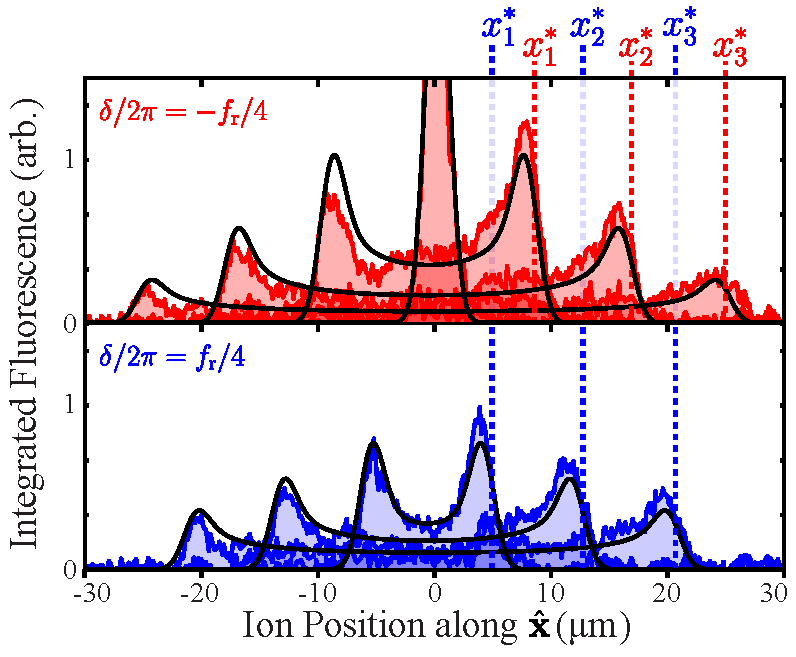
\includegraphics[width=1.0\columnwidth]{Column_Sums_06.pdf}
\end{center}
\caption{Integrated spatial images of fluorescence from an ion illuminated by an optical frequency comb whose nearest-resonant tooth is detuned to the red (upper) or blue (lower) of rest-frame resonance.  Multiple fixed points are shown (as individual traces) for each case.  Hysteresis associated with the ion's initial energy determines which fixed point the ion finds.  The dashed lines indicate the fixed-point oscillation amplitudes extracted from fitting to classical harmonic oscillator distributions (solid black curves). The systematic fluorescence asymmetry is due to the intensity gradient of the ML laser beam.}
\label{fig:ColumnSums}
\end{figure}

Figure \ref{fig:ColumnSums} shows the experimental signature of multiple fixed point solutions for the oscillation amplitude when the near-resonant tooth is red (upper) or blue (lower) detuned.  These integrated (along $\hat{\mathbf{y}}$) fluorescence images resemble the ``two-lobe'' shape of an image of a classical harmonic oscillator (or coherent state) probability distribution, shown as black curves.  The fits (which include convolution with our imaging system point-spread function) are used to extract the oscillation amplitude fixed points with a resolution-limited systematic uncertainty of $\pm 0.5 \mbox{ }\mu\mbox{m}$.  When the near-resonant tooth is red detuned, we find stable oscillation amplitudes $(x^\ast_1, x^\ast_2, x^\ast_3) = (8.6, 16.9, 25.0) \mbox{ }\mu\mbox{m}$, compared to the theoretical prediction of $(9.5, 18.0, 27.0)\mbox{ }\mu\mbox{m}$ from the roots of Eq.~\ref{eqn:PowerBalance}.  For the blue-detuned case, we find $(x^\ast_1, x^\ast_2, x^\ast_3) = (4.9, 12.7, 20.7) \mbox{ }\mu\mbox{m}$, with the corresponding predicted values $(5.2, 13.7, 22.4) \mbox{ }\mu\mbox{m}$ (see Fig.~\ref{fig:TheoryPowervsAmplitude}).  The measured fixed points agree with the predicted values to about $10$\%.

We further verified that the system behaves as a phonon laser amplifier by acoustically injection locking each of the first three fixed points (other than the $x_0^\ast \approx 0$ fixed point for $\delta<0$) for both signs of $\delta$ using the technique described in Ref. \cite{Knunz2010injection}, shown in Fig.~\ref{fig:InjectionLock}. Injection-locked phonon lasers of this sort may prove useful as sensitive force sensors \cite{Knunz2010injection} or test systems for models of quantum synchronization \cite{Lee2013quantum,Lee2014entanglement,Hush2015spin}.

\begin{figure}
\begin{center}
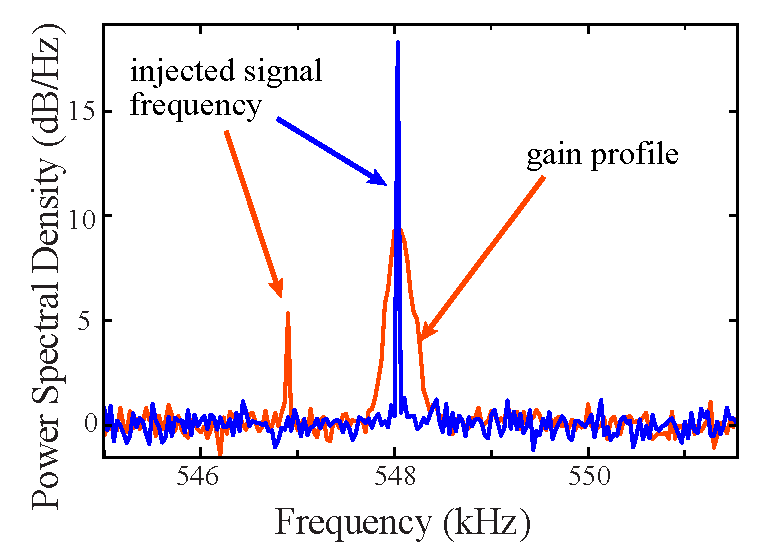
\includegraphics[width=1.0\columnwidth]{injection_lock_03.pdf}
\end{center}
\caption{Acoustic injection locking of the $x^\ast_1$ fixed point phonon laser when the near-resonant tooth is blue detuned.  When the frequency of an injected signal is moved from outside (orange) to within (blue) the phonon laser's gain bandwidth, it is amplified at the expense of other frequencies.}
\label{fig:InjectionLock}
\end{figure}

Both the theoretical model and the observed behavior we report here show that phenomena arising from inter-pulse coherence can still dominate ML-illuminated ion dynamics in the regime where $\tau < T_\mathrm{r}$.  For the Cd$^+$ laser cooling described in Ref.~\cite{Blinov2006broadband}, the probability of excited state decay between consecutive pulses was $P_\mathrm{decay}(\gamma, T_\mathrm{r})>98\%$, but Eq.~\ref{eqn:Visibility} shows that the limit on tooth visibility imposed by this decay is nonetheless $V=0.27$, and our model predicts stable fixed points with the lowest lying between $2 \mbox{ mK}$ and $2 \mbox{ K}$ in $E/k_\mathrm{B}$.  Single-pulse cooling effects can be added to our model by including an additional damping coefficient $\beta_\mathrm{env} \approx -(\hbar k/T_\mathrm{r})\, \partial_v P_\mathrm{ex}(\theta, kv)$ due to the slope of the single-pulse excitation probability envelope $P_\mathrm{ex}(\theta, kv)$ to Eq.~\ref{eqn:PowerBalance}, along with any technical heating rates, and solving for the steady-state energy.  As an estimate, for the lowest fixed point and in the absence of any technical heating, the pulse duration for which single-pulse cooling effects are comparable to comb effects will be near $\tau_\mathrm{pulse} \approx 2 T_\mathrm{r} V \approx 4\cos^2(\frac{\theta}{2})\, T_\mathrm{r} \,e^{-\gamma T_\mathrm{r}/2}$.

Since blue-detuned comb teeth do not pose an intractable problem for working with trapped ions, optical frequency combs may prove to be useful and robust tools for a variety of currently difficult species. In the case of $\mathrm{He}^+$, which is an attractive spectroscopic subject \cite{Herrmann2009feasibility}, $1\mbox{ mW}$ frequency comb light sources may soon become available at $\lambda \approx 61\mbox{ nm}$ \cite{Porat2017phase}, and 2-photon transitions could be used for slow Doppler cooling in the limit of low intensity \cite{Jayich2016direct}. Direct comb cooling of helium ions may then enable work with ${}^3\mathrm{He}^+$, the lightest atomic cation with an electron (and therefore the most difficult to sympathetically cool with another ion), where the ground state hyperfine splitting of $8.67\mbox{ GHz}$ \cite{Schuessler1969hyperfine} would easily be spanned by a comb for repumping and spectroscopy. We have tested one possible hyperfine repumping scheme for $I=1/2$ experimentally by laser cooling and repumping ${}^{171}\mbox{Yb}^+$ with only the ML laser, similar to the case recently reported for ${}^{25}\mathrm{Mg}^+$ \cite{DavilaRodriguez2016doppler}.

\begin{acknowledgments}
The authors acknowledge discussions with Boris Blinov and thank Eric Hudson for comments on the manuscript.  Technical assistance was provided by Sylvi Haendel and Danilo Dadic.  This work was supported by the U.S. Army Research Office under Grant No. W911NF-15-1-0261.  Initial work by A.M.J. and X.L. was supported by the NSF CAREER Program under award No. 1455357.
\end{acknowledgments}

M.I. and A.R. contributed equally to this work. The manuscript first draft was written by M.I. and W.C.C.  The data were taken by A.R., C.R., and M.I., with the initial observation of the phonon lasing aided by A.M.J. and X.L.
\bibliography{CombCoolingPhononLasing}
\end{document}
